\section{Umsetzung}

In diesem Kapitel wird der Lösungsweg für die im Pflichtheft aufgeführten Kriterien beschrieben.
Es ist anzumerken, dass die Kommentare im Quellcode teils in englischer Sprache verfasst sind. Grund dafür ist die Inkompatibilität des Latex-Listing-Pakets mit UTF8 Unicode Zeichen. Im Lösungsweg werden lediglich Ausschnitte des Quellcodes gezeigt. Die vollständigen Quellcodes befinden sich im Anhang.

\subsection{Einrichtung der Datenbank}

Als Grundlage für das Java-Ladeprogramm, der Ausführung der ETL-Skripte und der Prozedur zum Reporting für das DW müssen zunächst die Datenbanken eingerichtet und mit Daten befüllt werden. Die Einrichtung und Befüllung der Datenbanken werden mit Hilfe der zur Verfügung gestellten Skripte nach den vorliegenden Datenmodellen erstellt:

\begin{figure}[ht!]
  \centering
  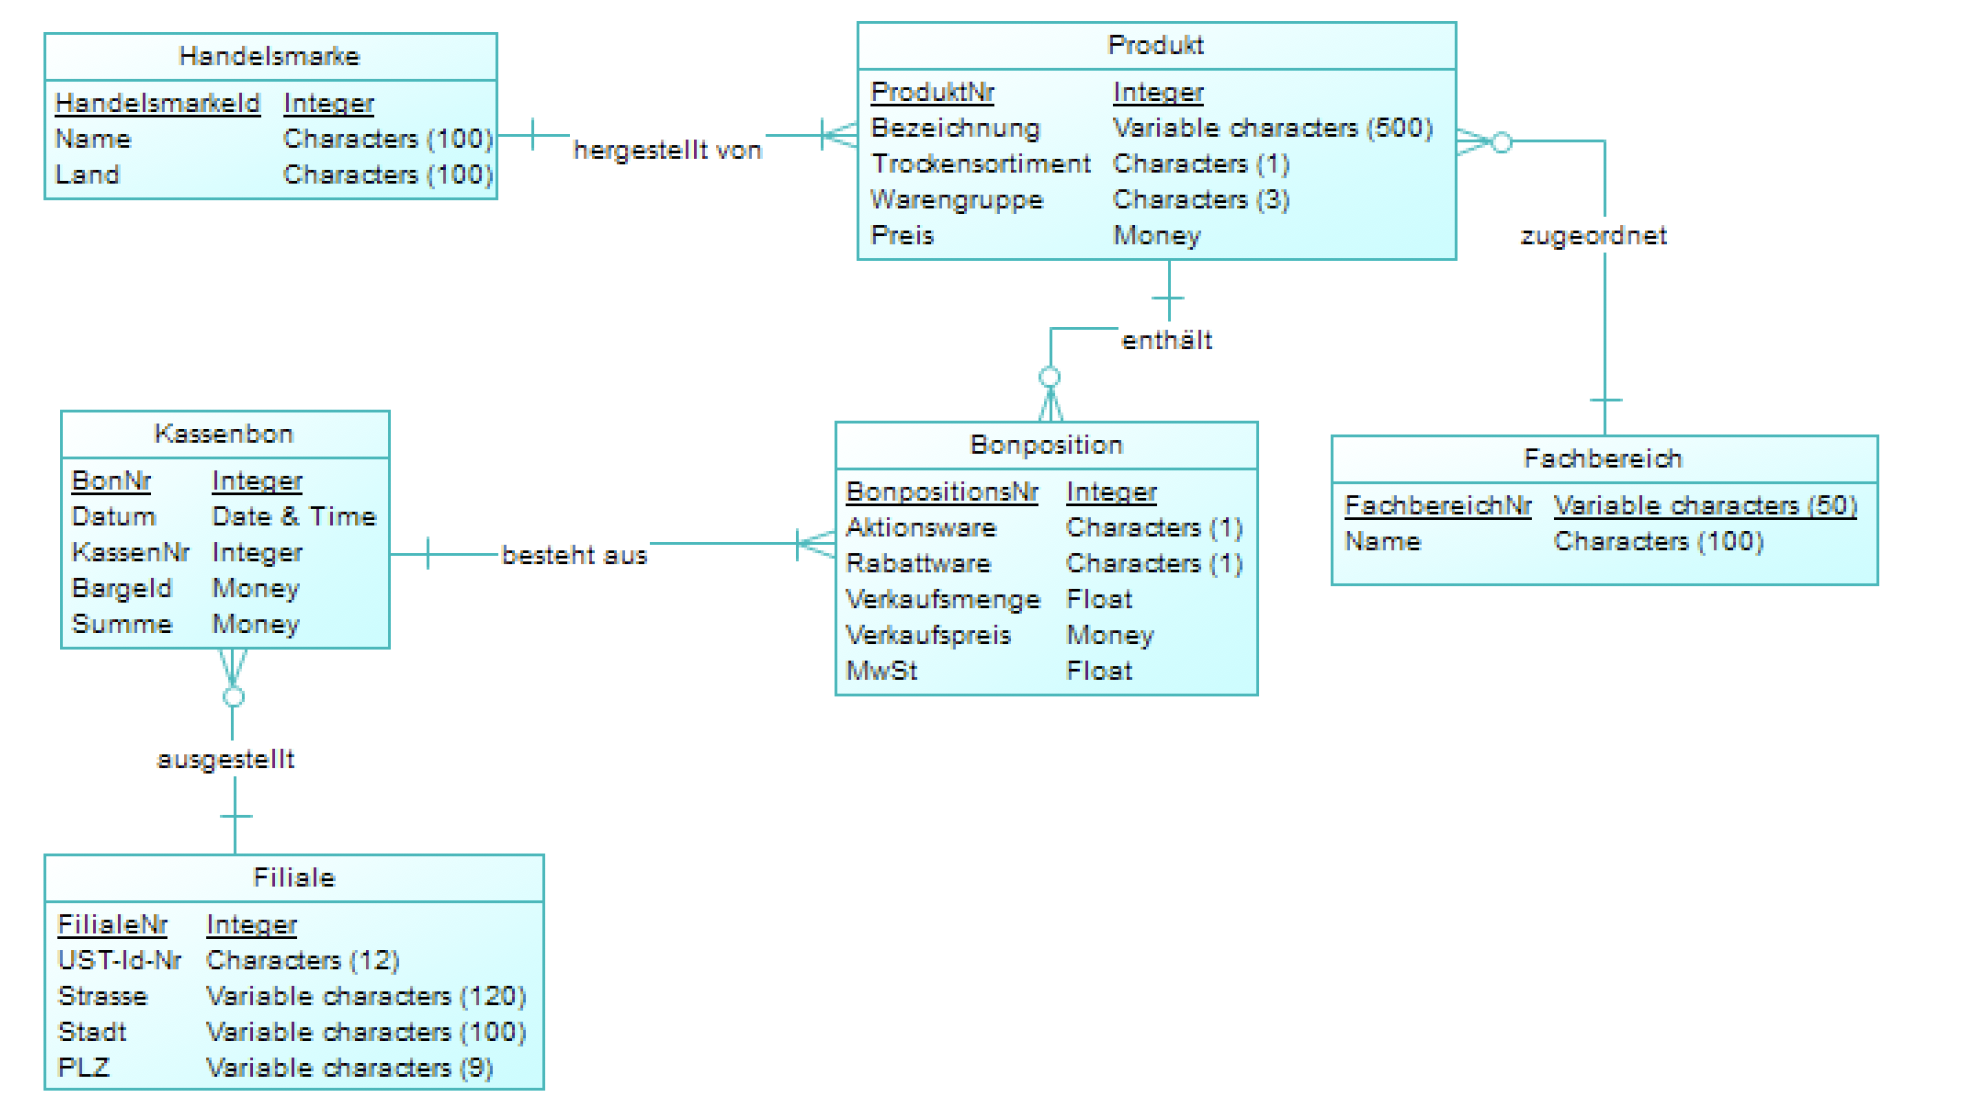
\includegraphics[width=1.2\linewidth]{pictures/db_basic.png}
  \caption[ER-Modell zur Auswertung von Kassenbons]{ER-Modell zur Auswertung von Kassenbons (Quelle: DBIS-Aufgaben)}
\end{figure}

\begin{figure}[ht!]
  \centering
  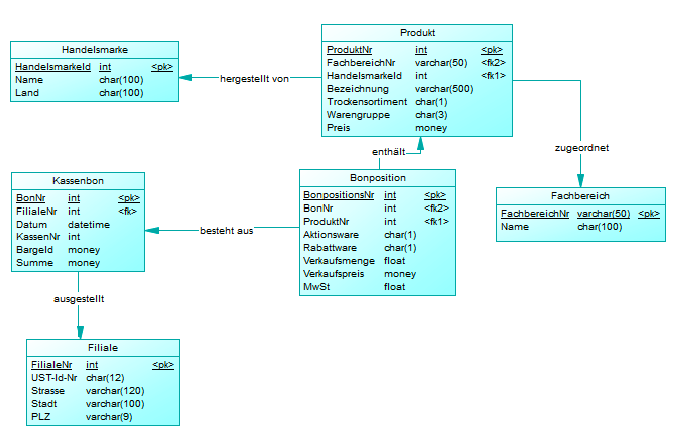
\includegraphics[width=1.2\linewidth]{pictures/phys_data.png}
  \caption[Physikalisches Datenmodell]{Physikalisches Datenmodell (Quelle: DBIS-Aufgaben)}
\end{figure}

\subsection{Java-Programm}

Das Java-Programm soll dazu dienen, den Datenbestand für Produkte aus der CSV-Datei \textbf{PRODUKTE.1} zu erweitern. Allerdings ist die Datei von fehlerhaften Daten befallen, welche nicht mit der Struktur der Datenbanktabelle übereinstimmen. Um diese Problematik zu lösen, wurde mit Hilfe des zur Verfügung gestellten Ladeprogramms ein eigenes Programm entwickelt. Einige Klassen wurden komplett selbst enwickelt und andere angepasst, während die Klasse \textbf{DateFormat} vollständig übernommen wurde.
Zunächst wurde ein Importfenster (s. Abbildung \ref{import}) mit der Klasse \textbf{ImportWindow} erzeugt. Es dient dazu, die Parameter für die Verbindung mit dem Datenbankserver einzutragen und die zu hochladende CSV-Datei aus dem Computerverzeichnsi auszuwählen. Ob die Datenbankverbindung erfolgreich war, wird in dieser Klasse getestet. Die durchgeführten Aktionen werden in dem Protokoll dokumentiert. Man kann daraus entnehmen, welche Zeilen der Datei erfolgreich geladen wurden und welche aus welchem Grund fehlgeschlagen sind.
\begin{figure}[ht!]
  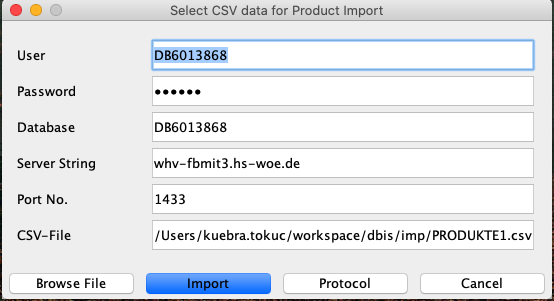
\includegraphics[width=1\linewidth]{window.png}
  \caption{Importfenster des Java-Programms}
  \label{import}
\end{figure}
Die Datenbankverbindung wird in der Klasse \textbf{DBConnection} eingerichtet. Im Gegesatz zu der Implementierung im Beispielprogramm, wurde in diesem Beispiel ein \textbf{JDBC Data Source} Objekt verwendet, welches den gleichen Treiber verwendet wie das Beispielprogramm. Der Grund für die Entscheidung ist die zum Einen die Übersichtlichkeit und zum anderen die Tatsache, dass diese Herangehensweise mittleweile bevorzugt sei \citep{Wulff2019}.

\begin{lstlisting}
  public synchronized Connection getConnection() throws SQLException{

		// Connection with DataSource

		try {
			if (con == null || con.isClosed()) {
				DataSource ds = new TdsDataSource();
				((TdsDataSource) ds).setServerName(serverName);
				((TdsDataSource) ds).setPortNumber(Integer.parseInt(port));
				con = ds.getConnection(username, password);
				con.setCatalog(databaseName);
			}
		} catch (SQLException e) {
			log.log(Level.WARNING, "DB Connection failed.", e);
			JOptionPane.showMessageDialog(new JFrame(),
					" DB Connection failed!\n" +
							"Check your connection input",
							"CSV Import", JOptionPane.ERROR_MESSAGE);
		}
		return con;

	}
\end{lstlisting}

Die Klasse \textbf{FileLineParser} für die Erzeugung eines Objekts für den Import wurde ebenfalls angepasst und erweitert. Zum Beispiel werden die Warengruppennummern und Fachbereichsnummern mit übergeben, damit sie nicht nachträglich angepasst werden müssen. Zudem wird eine Methode zum Erstellen eines neuen Fachbereichs in der DB für Gewürze angestoßen, damit die Zuordnung korrekt stattfindet. Die Methode \textbf{isDub} prüft, in einer Hashmap, ob Einträge in einer Zeile redundaten ist und gibt bei Redundanzen den Wert true zurück. Dies ist für die Fehlerbehandlung von großer Bedeutung.

\begin{lstlisting}
  // Ubergabe der Warengruppennummer

	public static String getWarengruppe(String s_warengruppe) {

		if (s_warengruppe == null)
			return null;

		String warengruppe_id = null;

		if (s_warengruppe.equalsIgnoreCase("Milch"))
			warengruppe_id = "002";
		else if (s_warengruppe.equalsIgnoreCase("Musli & Cerealien"))
			warengruppe_id = "003";
		else if (s_warengruppe.equalsIgnoreCase("Saucen"))
			warengruppe_id = "004";
		else if (s_warengruppe.equalsIgnoreCase("Gewurze"))
			warengruppe_id = "005";
		else
			warengruppe_id = "006";

		return warengruppe_id;
	}

	// Ubergabe der Fachbereichsnummer
	// wird auch Fachbereich fuer Gewurze erstellen

	public static String getFachbereichsNummer(String warengruppe_id) throws SQLException {

		if (warengruppe_id==null) {
			return null;
		}
		String fb_id= null;
		if (warengruppe_id=="002") {
			fb_id= "1014";
		}else if(warengruppe_id == "003") {
			fb_id= "1023";
		}else if(warengruppe_id == "004") {
			fb_id= "1015";
		}else if(warengruppe_id == "005") {
			ImportRoutine.createNewFB("Gewurze", "1039");
			fb_id="1039";
		}

		return fb_id;
	}

	// Methode zum Prufen von Redundanten Eintragen

	public static boolean isDub(String bezeichnung) {

		String[] words = bezeichnung.split("[\\s+]");

		Map<String, Integer> occurrences = new HashMap<String, Integer>();

		boolean isdub =false;
		Integer oldCount=0;
		for ( String word : words ) {
			oldCount = occurrences.get(word);
			if ( oldCount == null ) {
				oldCount = 0;
			}
			occurrences.put(word, oldCount + 1);
			if(oldCount>2) isdub = true;
			System.out.println("oldcount : "+ oldCount+ "word"+ word + "isdub" + isdub);
		}
		System.out.println("IS DUB? :"+ isdub);
		return isdub;
	}

}
\end{lstlisting}

Die Klasse \textbf{ImportRoutine} wurde ebenfalls angepasst. Zudem wurde eine Methode zum Erzeugen eines neuen Fachbereichs hinzugefügt.
In \textbf{DBImport} findet die Ausführung der Datenbanktransaktionen statt. Auch der Insert des Fachbereichs findet hier statt.

\begin{lstlisting}
  public static void createNewFB(String name, String fb_nr) throws SQLException {

        DBImport.insertFB(name, fb_nr, con);

      }
\end{lstlisting}

\subsection{Data Warehouse}

\subsubsection{Erweiterung des Datenbestandes}
Da in Datenanalysen die Menge der Daten einen wichtigen Einfluss hat, wird der Datenbestand um 9 Handelsmarken, 9 Fachbereiche, 40 Kassenbons mit je 3 Bonpositionen erweitern. Die Verkaufspreise Summen im Kassenbon sind zu diesem Zeitpunkt noch nicht auf die Beträge der Bonpositionen angepasst und sind \glqq Dummy-Werte\grqq{}

\begin{lstlisting}[language=SQL]

  --- Beispiel fur einige Kassenbons ---
  insert into KASSENBON (FILIALENR, DATUM, KASSENNR, BARGELD, SUMME)
VALUES

(14, CONVERT([datetime], '2019-02-10 08:22:00.000', 20), 1, 400.00, 400.00),
(14, CONVERT([datetime], '2019-02-11 10:22:00.000', 20), 1, 33.00, 33.00),
(14, CONVERT([datetime], '2019-02-16 08:22:00.000', 20), 1, 12.00, 12.00),
(14, CONVERT([datetime], '2019-02-17 10:22:00.000', 20), 1, 123.00, 150.00),
--- Beispiel fur Bonpositionen des Bons Nr. 10 ---
insert into BONPOSITION (BONNR, PRODUKTNR, AKTIONSWARE, RABATTWARE, VERKAUFSMENGE, VERKAUFSPREIS, MWST)
values
(10, 1, 'N', 'N', 1, 12.79, 12.79 * 0.07),
(10, 2, 'N', 'N', 1, 11.9900, 11.9900 * 0.07),
(10, 3, 'Y', 'Y', 10, 24.900, 24.900 * 0.07);

--- Hinzufugen von Handelsmarken ---
insert into HANDELSMARKE (NAME, LAND)
values
('Schar', 'Deutschland'),
('Nestle', 'Schweiz'),
('Kellog''s', 'USA'),
('Coca Cola', 'USA'),
('Goutess', 'Deutschland'),
('Gutfried', 'Deutschland'),
('Jever', 'Deutschland'),
('Nick', 'USA'),
('Basic', 'USA');

-- ** Gewurze wurden bereits aus dem Java-Programm heraus hinzugefugt *** --
insert into FACHBEREICH (FACHBEREICHNR, NAME)
values
(1040,'Snacks'),
(1041,'Oriental'),
(1042,'Asia'),
(1043,'Italienisch'),
(1044,'Drogerie'),
(1045,'Haushalt'),
(1046,'Getranke'),
(1047,'Desserts');
(1048,'Tierfutter');

\end{lstlisting}
\subsubsection{Aufbereitung des Datenbestandes}

Es wurden zwar Daten hinzugefügt, aber waren noch nicht den richtigen Handelsmarken zugeordet. Daher wurde gepüft, welche Handelsmarken ID der Produktbezeichnung zugefügt werden soll.
Außerdem wurde die Summe der Kassenbons nachträglich aus der Summe der Verkaufspreisen der einzelnen Bonpositionen korrigiert. Damit das Bargeld höher ist als die Summe, wurden standardmäßig 50 Euro addiert.

\begin{lstlisting}[language=SQL]
  -- *** Beispiel Zuordnung der Handelsmarken *** --

update PRODUKT
set HANDELSMARKEID = 40
where BEZEICHNUNG LIKE '%Kellog%';

update PRODUKT
set HANDELSMARKEID = 42
where BEZEICHNUNG LIKE '%Goutess%';

-- ** Update der Summen in Kassenbons ** --

UPDATE KASSENBON
SET SUMME = t.summe_einkauf
FROM KASSENBON AS kb
INNER JOIN
    (
        SELECT BONNR, SUM(VERKAUFSPREIS) summe_einkauf
        FROM BONPOSITION
        GROUP BY BONNR
    ) t
    ON t.BONNR = kb.BONNR

-- ** Bargeld an Summe anpassen, um Deckung zu gewaehrleisten ** --

update KASSENBON
	set BARGELD = Round(SUMME, 0)

-- ** Bargeld standardmaessig erhoehen, um Differenz zu erzeugen ** --

update KASSENBON
	set BARGELD = BARGELD + 50

-- ** runden ** --

update KASSENBON
	set BARGELD = Round(Bargeld,-1)


\end{lstlisting}

\subsubsection{Analyse des Starschemas}

Nachdem der Datenbestand erweitert und korrekt aufbereitet worden ist, wird ein Star-Schema für ein Data-Warehouse zur Umsatzanalyse und Auswertung von Verkaufsdaten nach einem vorliegenden Schema (s. Abbildung \ref{dw_concept}) erstellt. Das Star-Schema besteht aus Dimensionen- und Faktentabellen, welche die Struktur und den Inhalt einer multidimensionalen Datenmenge definieren \citep{Wulff2019}. Die Werte in der Faktentabelle werden durch die Primary Keys der Dimensionstabelle mit ihr in Abhängigkeit gebracht (s. Abbildung \ref{dw_phys}). Allerdings ergibt die Analyse des Datenmodells Inkosistenzen zwischen den verschiedenen Tabellen:

\begin{enumerate}
  \item Kein Fachbereich im Sternschema, stattdesen Abteilung
  \item Kassenbon\_Fakten AbteilungsNr FK int und DIM\_Abteilung AbteilungsNr PK int
  \item FilialeNr int der operativen DB und FilialeNr char(3) der DIM\_Filiale
  \item Warengruppe char(3) der operativen DB (ODB) und Warengruppe char(1) der DIM\_Produkt
  \item Bezeichnung des Produkts in ODB varchar(500) und in DIM\_Produkt varchar(100)
\end{enumerate}

Es stellte sich jedoch heraus, dass diese Unterschiede keinen Einfluss auf den Report hatten.

\begin{figure}[ht!]
  \centering
  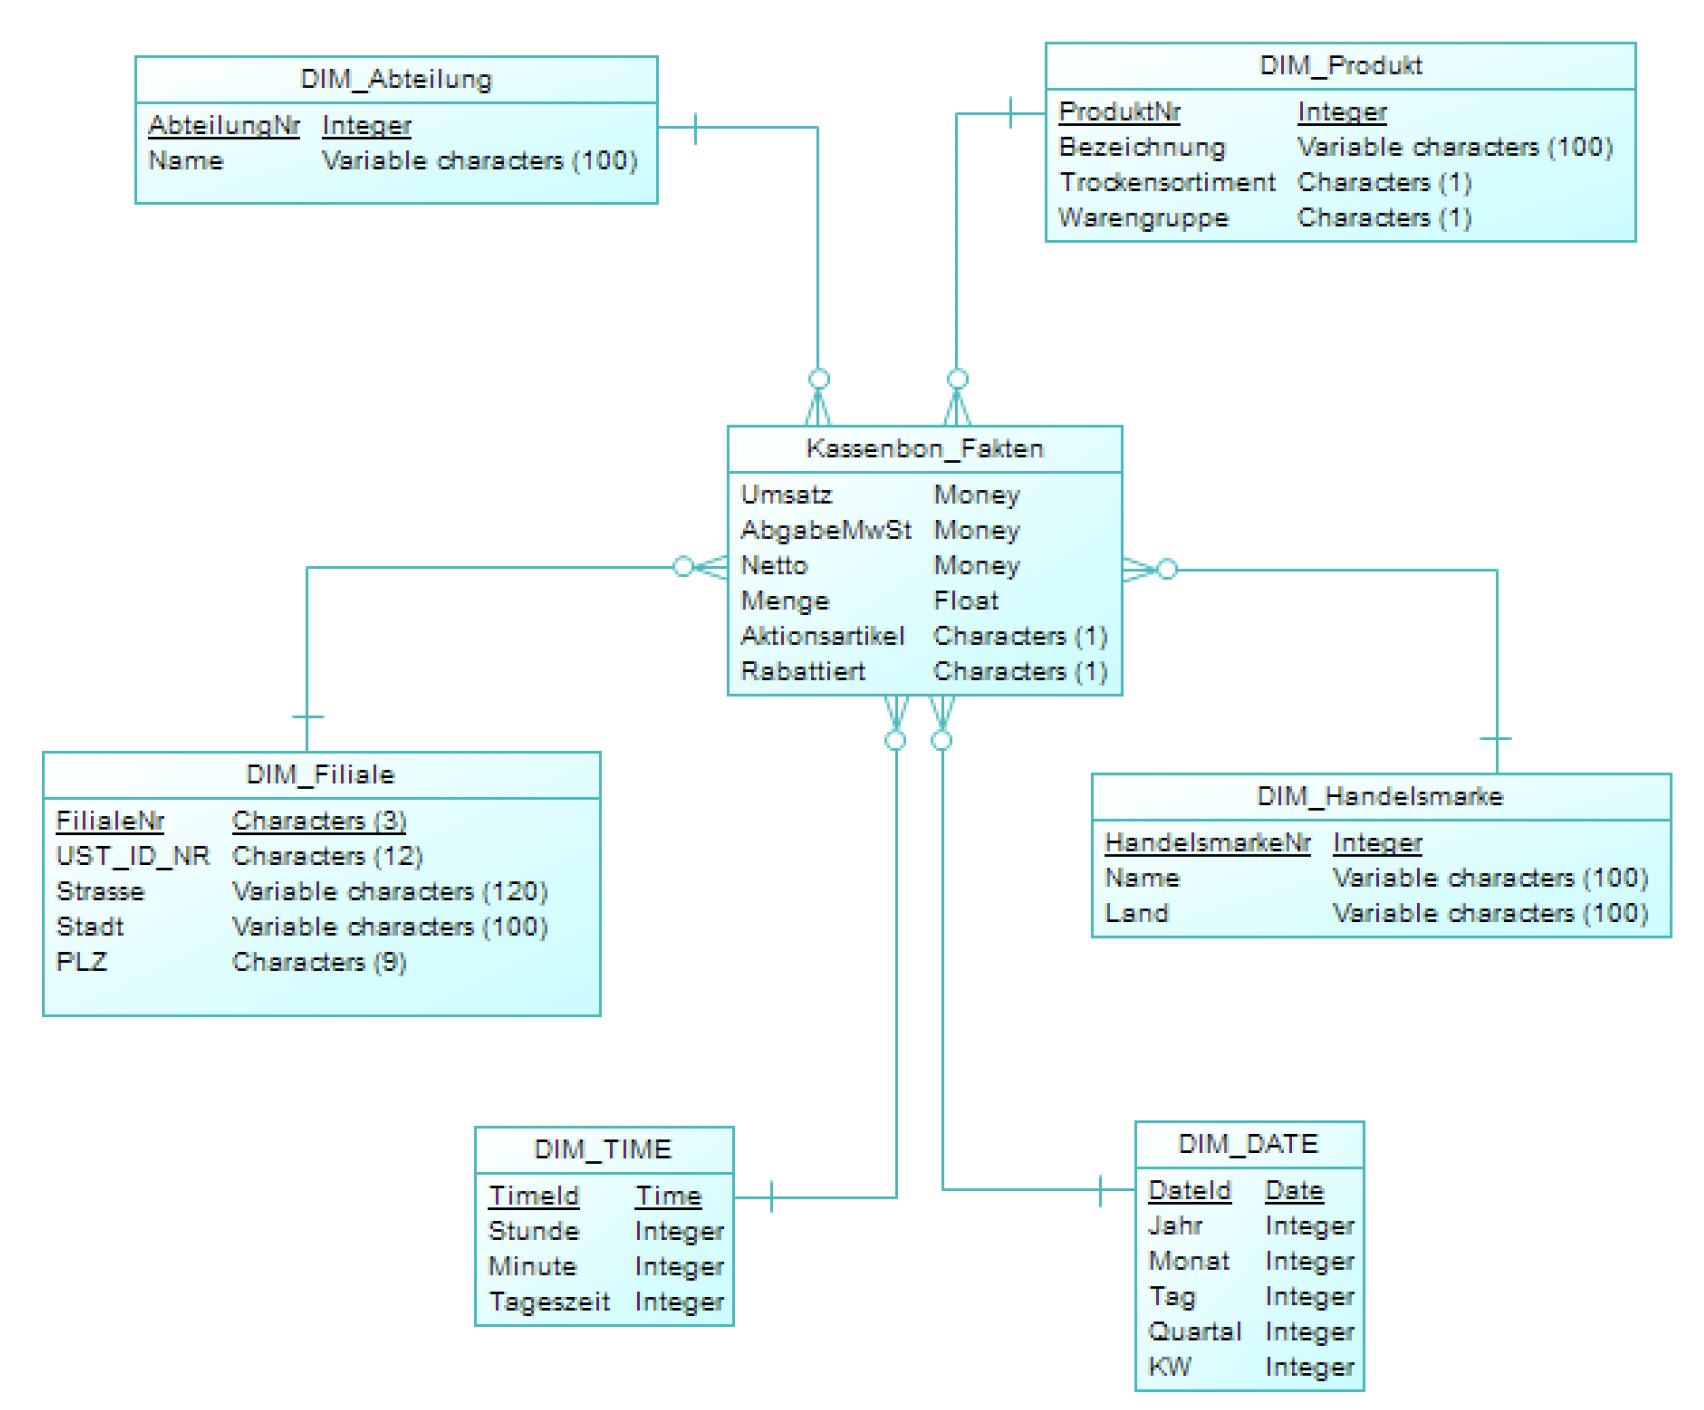
\includegraphics[width=1.1\linewidth]{pictures/dw_concept.png}
  \caption[Konzeptionelles Datenmodell des Data-Warehouses]{Konzeptionelles Datenmodell des Data-Warehouses (Quelle: DBIS-Aufgaben)}
  \label{dw_concept}
\end{figure}

\begin{figure}[ht!]
  \centering
  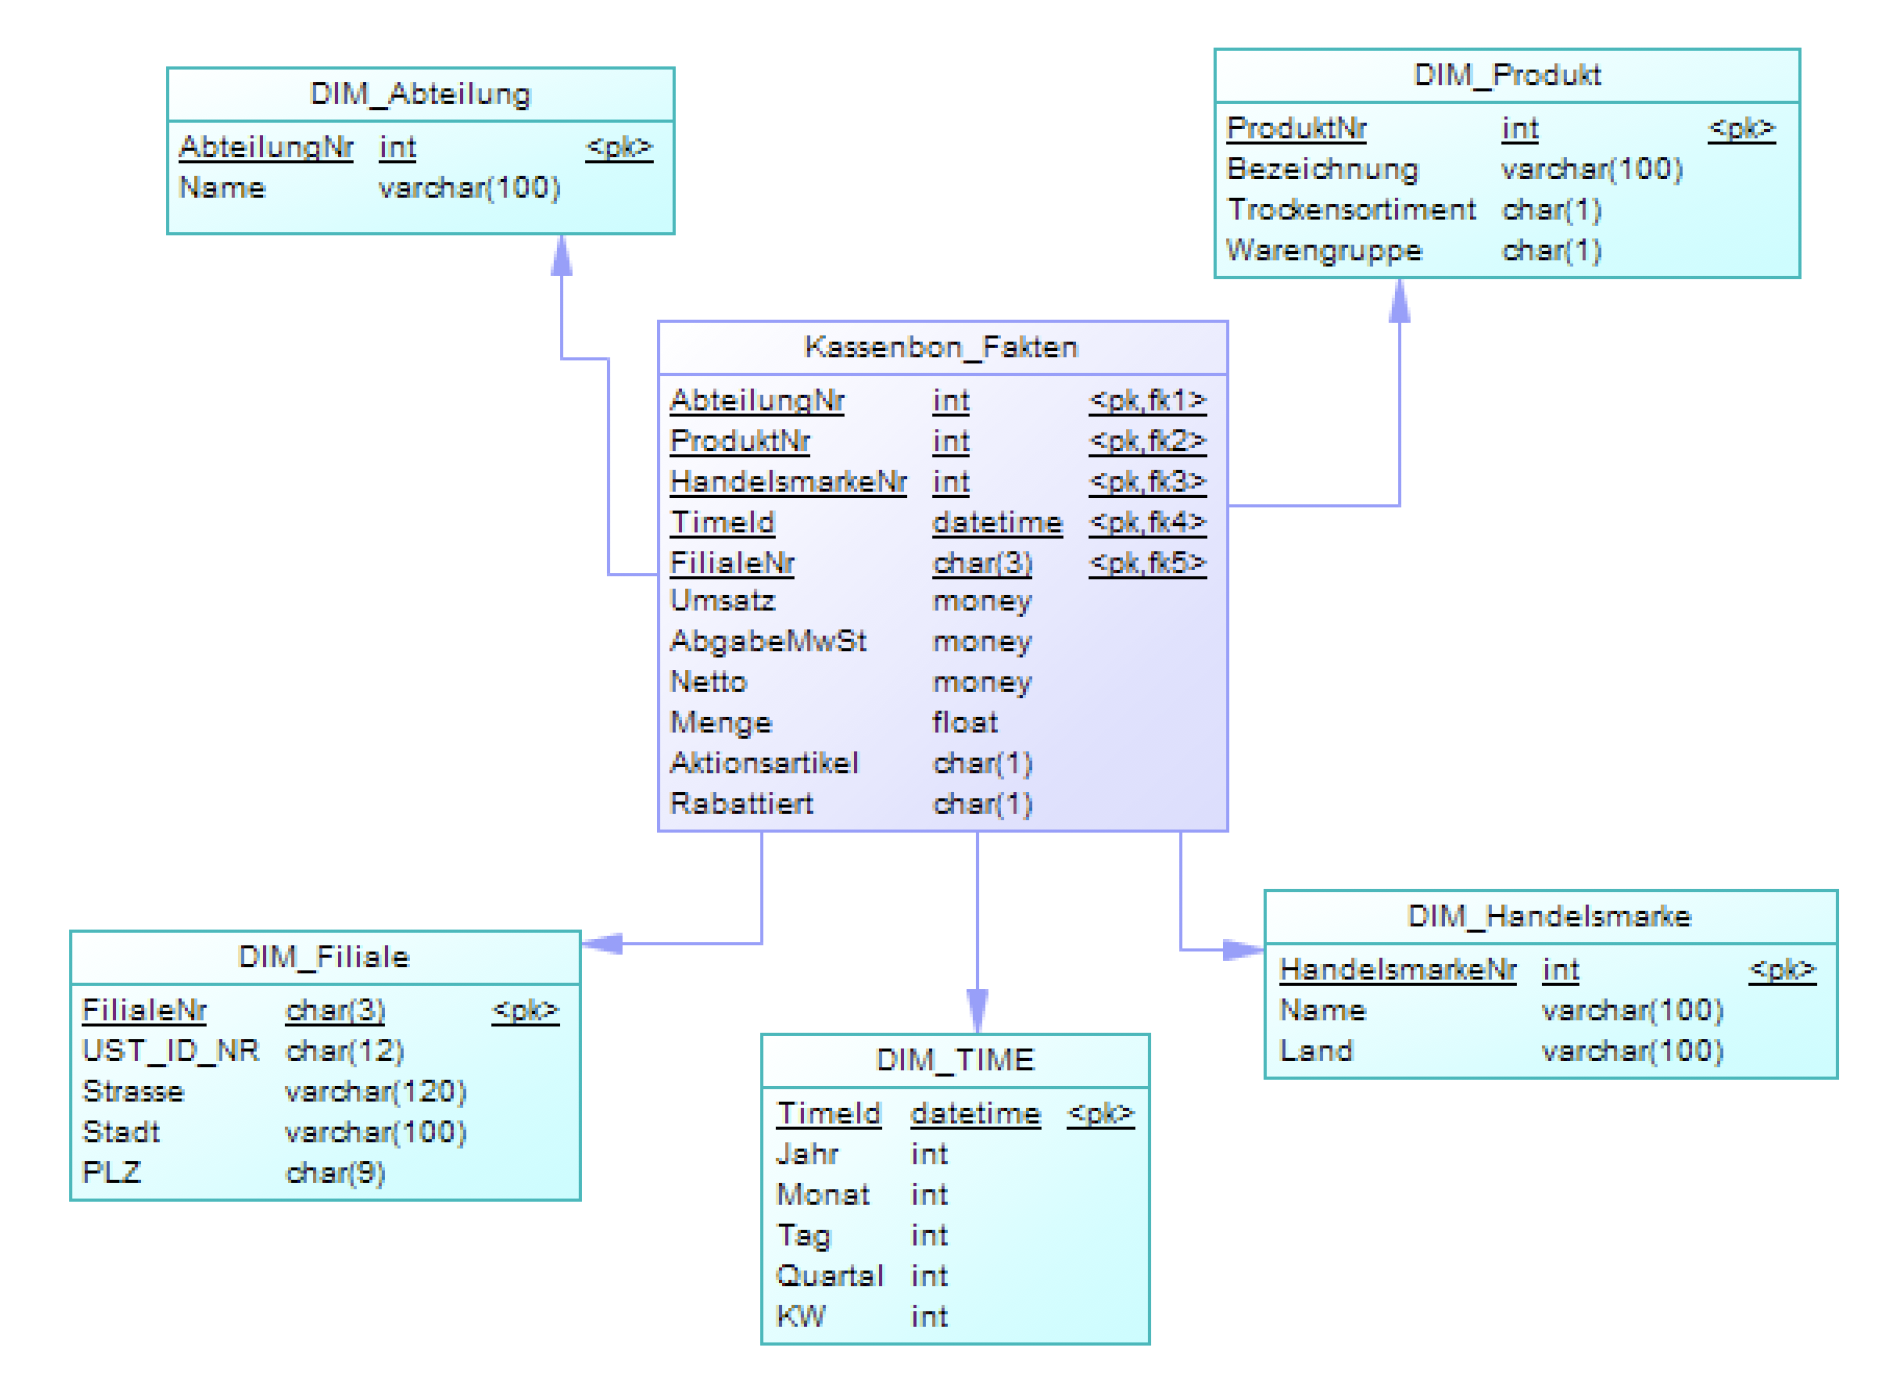
\includegraphics[width=1.1\linewidth]{pictures/DW_Physical_Data.png}
  \caption[Physikaliches Datenmodell des Data-Warehouses]{Physikaliches Datenmodell des Data-Warehouses (Quelle: DBIS-Aufgaben)}
  \label{dw_phys}
\end{figure}

\begin{figure}[ht!]
  \centering
  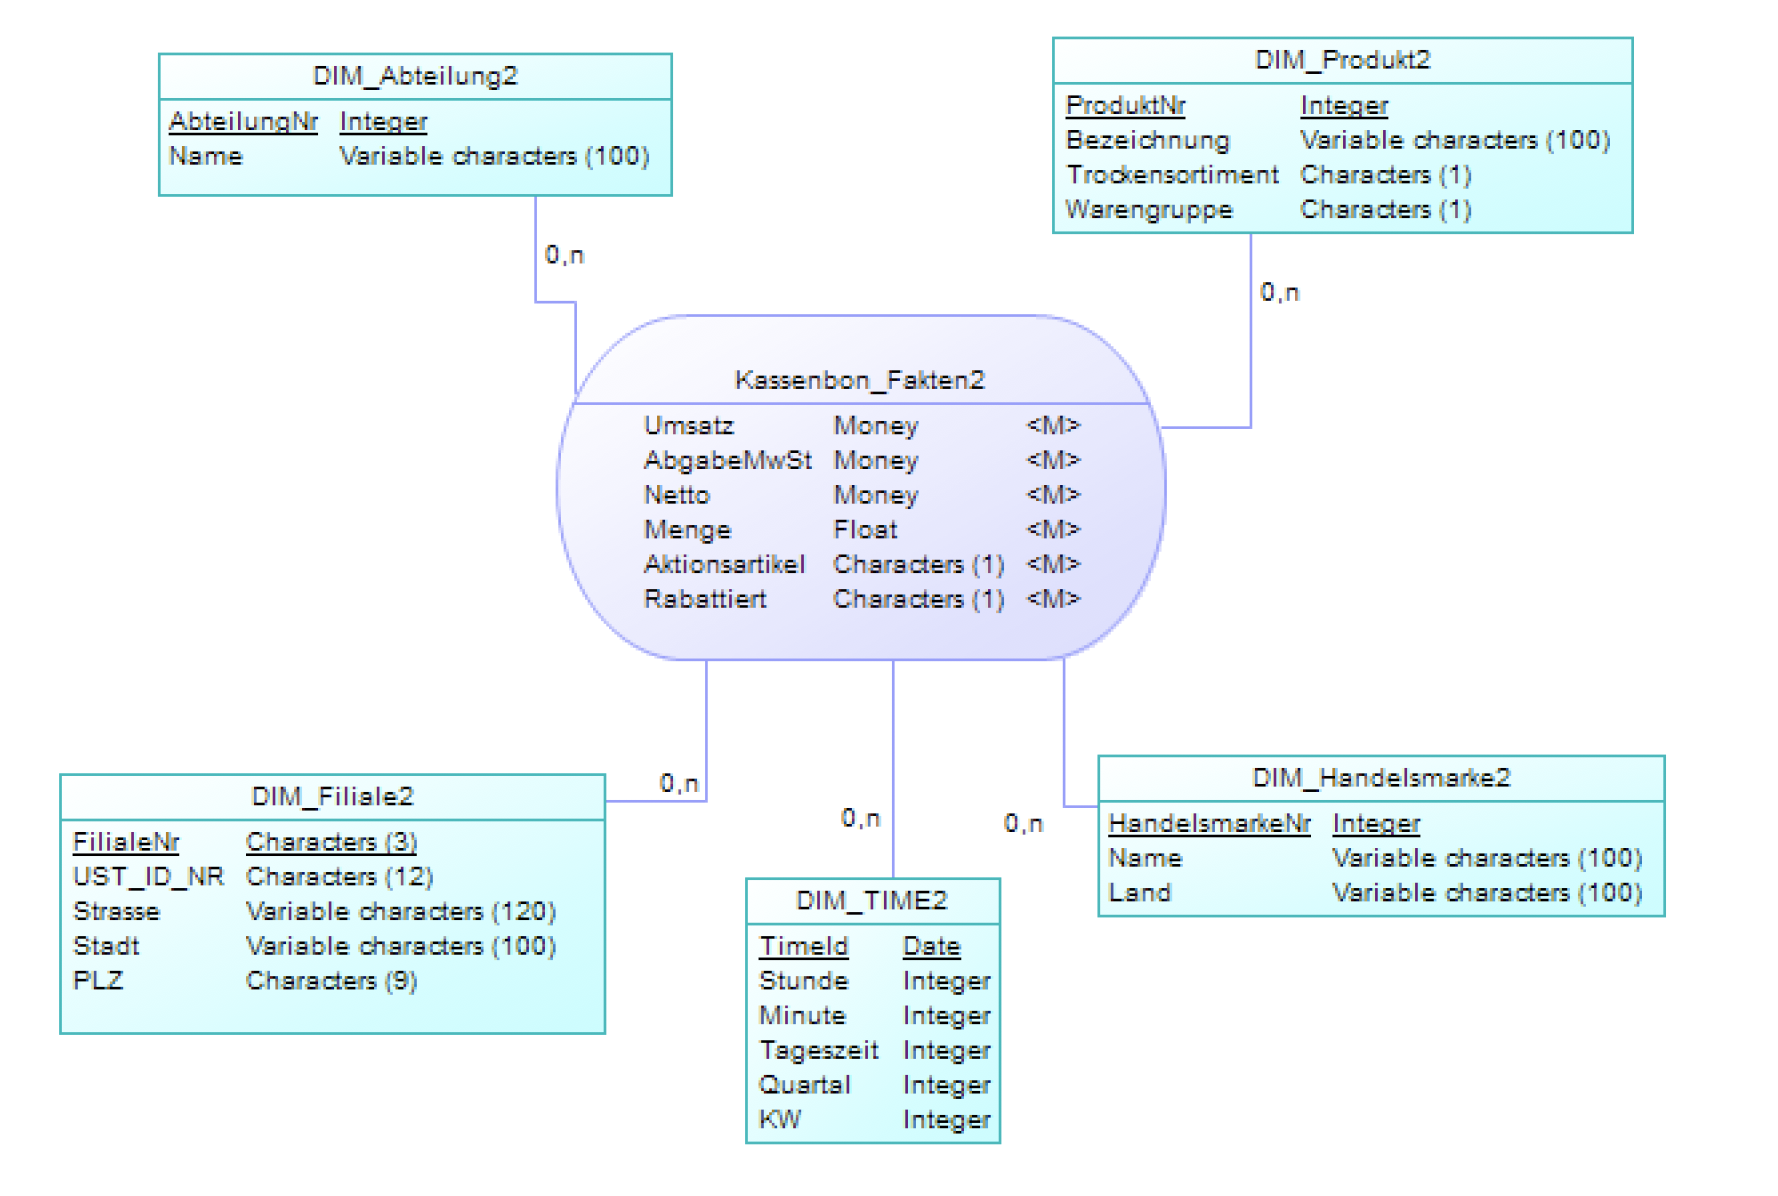
\includegraphics[width=1.1\linewidth]{pictures/dw_asso.png}
  \caption[Datenmodell des DW mit Assoziierung]{Datenmodell des DW mit Assoziierung (Quelle: DBIS-Aufgaben)}
  \label{dw_asso}
\end{figure}

\subsubsection{ETL-Prozess}

Mit dem ETL-Prozess (Extract, Transform, Load) werden die Daten aus der operativen Datenbank für die Auswertung und Analyse aufbereitet und in das Data Warehouse geladen. Weil die Fremdschlüssel und Primärschlüssel der Faktentabelle für Kassenbons aus den Primärschlüsseln der Dimensionstabellen bestehen (s. Abbildung \ref{dw_phys}), müssen zunächst Insert-Anweisungen für die Dimensionstabellen ausgeführt werden.

\begin{lstlisting}[language=SQL]
  -- Dim-Tabellen mit Werten aus der ODB befullen --
--DIM_Abteilung--
insert into DIM_Abteilung(AbteilungNr,Name)
select FB.FachbereichNr,FB.Name
from Fachbereich as FB

--DIM_Produkt--
insert into DIM_PRODUKT(PRODUKTNR,BEZEICHNUNG,TROCKENSORTIMENT,WARENGRUPPE)
select P.ProduktNr, P.Bezeichnung, P.Trockensortiment, substring(P.Warengruppe,3,1)
from Produkt as P

--DIM_Filiale--
insert into DIM_FILIALE(FILIALENR, UST_ID_NR,STRASSE,STADT,PLZ)
select F.FILIALENR,F.UST_ID_NR, F.STRASSE,F.STADT, F.PLZ
from FILIALE as F

--DIM_Handelsmarke--
insert into DIM_HANDELSMARKE(HANDELSMARKENR,NAME, LAND)
select HM.HANDELSMARKEID, HM.NAME, HM.LAND
from HANDELSMARKE AS HM
\end{lstlisting}

Im Anschluss kann die Dimensionstabelle DIM\_Date auf den Tag, die Woche, den Monat, das Quartal und das Jahrgenau gespeichert werden. Dafür wird das vom Anfangsdatum bis zum Endatum der Kassenbons eine Schleife durchlaufen. Die Dim\_Time läuft auf ähnliche Weise, nur dass die Schleife einen ganzen Tag durchläufz und ihn in Zeitabschnitte unterteilt.

\begin{lstlisting}[language=SQL]
  -DIM_Date Parameter fur die Berechnung der Attribute--
--Alle Tage von Anfang bis Ende ---
declare @vonDatum date,
		@bisDatum date,
		@Jahr integer, -- Attribut "Jahr"
		@Monat integer, -- Attribut "Monat"
		@Tag integer, -- Attribut "Tag"
		@Quartal integer, -- Attribut "Quartal"
		@KW integer -- Attribut "Kalenderwoche"

	select @vonDatum=min(CONVERT(date,datum)) from KASSENBON
	select @bisDatum=max(CONVERT(date,datum)) from KASSENBON

-- Zeitspanne: Schleife, bis Enddatum Erreicht wurde --

	while @vonDatum <= @bisDatum
		begin
			set @Jahr		=year(@vonDatum)
			set @Monat		=month(@vonDatum)
			set @Tag		=day(@vonDatum)
			set @Quartal	=datepart(Quarter,@vonDatum)
			set @KW			=datepart(WK,@vonDatum)

			insert into DIM_DATE(DATEID, JAHR, MONAT, TAG, QUARTAL, KW)
			values (@vonDatum, @jahr, @monat, @tag, @Quartal, @KW)

		set @vonDatum = DATEADD(DD, 1,@vonDatum)
	end
\end{lstlisting}

Zum Schluss findet der Insert der Kassenbonfakten durchgeführt werden. Dafür werden die Primärschlüssel der operativen DB gejoined. Mit dem Insert der Zeitdimensionen kann die Faktentabelle zum Beispiel das Verkaufsdatum auf das Produkt beziehehen oder Umsätze nach Produkt generieren. Zu beachten war außerdem, die Differenz zwischen der summierten Verkaufspreise und der Mehrwertsteuern zu erzeugen, um einen Nettobetrag zu erhalten.

\begin{lstlisting}[language=SQL]

  --- Insert der Kassenbon_Fakten ---
  INSERT INTO KASSENBON_FAKTEN
	select fbr.FACHBEREICHNR, P.PRODUKTNR, hm.HANDELSMARKEID,
	convert(date,DATEID), convert(time(0),TIMEID),
    F.FILIALENR, sum(BP.Verkaufspreis), sum(BP.MWST),
	sum(BP.Verkaufspreis)  - sum(BP.MWST),
	sum(BP.Verkaufsmenge),
	bp.AKTIONSWARE,
  bp.RABATTWARE

  --- Gruppierung der Faktentabelle nach: -----
  group by
	fbr.FACHBEREICHNR, P.PRODUKTNR, hm.HANDELSMARKEID,
	DD.DATEID, DT.TIMEID, F.FILIALENR,
  BP.AKTIONSWARE, BP.RABATTWARE,BP.BONNR

\end{lstlisting}

\subsubsection{Aggregate auf Wochenbasis}

Um Aggregate auf Wochenbasis zu erhalten, wurde auf ähnliche Weise wie die Faktentabelle für Kassenbons eine Faktentabelle für Kassenbons auf Wochenbasis erstellt. Sie stellt dar, in welchen Wochen der meiste Umsatz mit welchem Produkt und welcher Menge erzielt worden ist.

\begin{figure}[ht!]
  \centering
  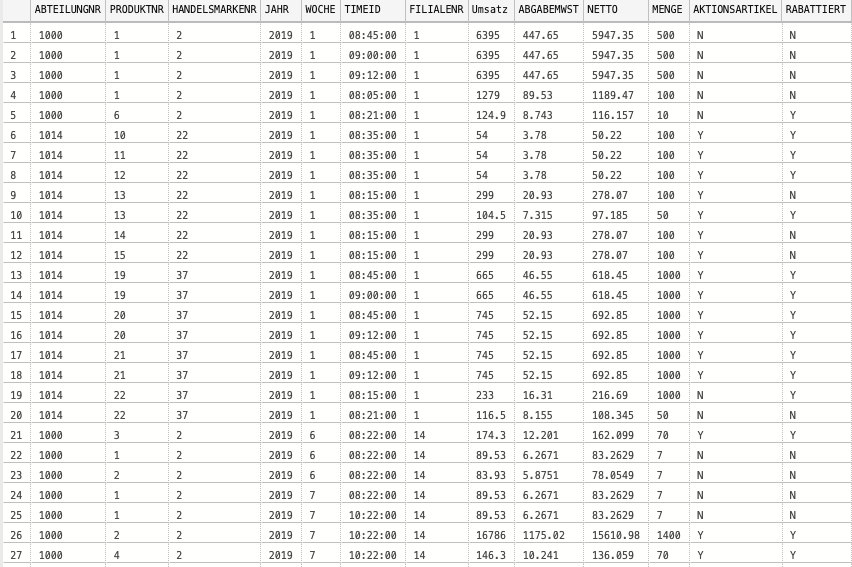
\includegraphics[width=1.1\linewidth]{pictures/fakten_woche.png}
  \caption{Aggregate auf Wochenbasis}
  \label{fakten_woche}
\end{figure}

\begin{lstlisting}[language=SQL]
  INSERT INTO KASSENBON_FAKTEN_WOCHEN
	select
	FB.FACHBEREICHNR, P.PRODUKTNR,	H.HANDELSMARKEID,
	DD.JAHR, DD.KW, convert(time(0),TIMEID),
	F.FILIALENR, sum(BP.Verkaufspreis),
	sum(BP.MWST), sum(BP.Verkaufspreis)-sum(BP.MWST),
	sum(BP.Verkaufsmenge), BP.AKTIONSWARE, BP.RABATTWARE
	from
	FACHBEREICH as FB join Produkt as P
		on FB.FACHBEREICHNR= P.FachbereichNr join
HANDELSMARKE as H
		on P.HandelsmarkeId = H.HANDELSMARKEID
	join Bonposition as BP on P.ProduktNr = BP.ProduktNr
	join Kassenbon as KB on BP.BonNr = KB.BonNr
	join FILIALE as F on KB.FilialeNr = F.FILIALENR
  join Dim_Date as DD on DATEPART(yyyy,KB.Datum) = DD.JAHR and
  DATEPART(wk,KB.DATUM) = DD.KW
	join Dim_Time as DT on convert(time(0),KB.Datum) = DT.TIMEID
	group by
	FB.FACHBEREICHNR,
	P.PRODUKTNR,
	H.HANDELSMARKEID,
	DD.JAHR,
	DD.KW,
    DT.TIMEID,
	F.FILIALENR,
	BP.AKTIONSWARE,
	BP.RABATTWARE
\end{lstlisting}

\subsection{Zugänglichkeit für die Öffentlichkeit}

Mit dem folgenden Skript können auch weitere DB-Teilnehmer auf die Datenbanktabellen zugreifen, indem die Tabellen auf Public gesetzt werden.

\begin{lstlisting}[language=SQL]
  - Datentabellen/DB freigeben --

  GRANT CONNECT to public


  GRANT SELECT ON dbo.FILIALE to public
  GRANT SELECT ON dbo.KASSENBON to public
  GRANT SELECT ON dbo.BONPOSITION to public
  GRANT SELECT ON dbo.PRODUKT to public
  GRANT SELECT ON dbo.FACHBEREICH to public
  GRANT SELECT ON dbo.HANDELSMARKE to public

  GRANT SELECT ON dbo.DIM_TIME to public
  GRANT SELECT ON dbo.DIM_DATE to public
  GRANT SELECT ON dbo.DIM_ABTEILUNG to public
  GRANT SELECT ON dbo.DIM_PRODUKT to public
  GRANT SELECT ON dbo.DIM_FILIALE to public
  GRANT SELECT ON dbo.DIM_HANDELSMARKE to public
  GRANT SELECT ON dbo.KASSENBON_FAKTEN to public
  GRANT SELECT ON dbo.KASSENBON_FAKTEN_WOCHEN to public
  GRANT SELECT ON dbo.DW_REPORT_TABLE to public

  GRANT EXECUTE ON dbo.DW_REPORT to public
\end{lstlisting}

\subsection{Prozedur für das Reporting}
Um die Daten aus dem Data Warehouse in der Konsole eines SQL-Editors auszuwerten, kann eine Prozedur entwickelt werden. Prozeduren mit der Prozesdursprache TSQL verhalten sich ähnlich wie Methodenaufrufe in Java. Mit einem \textbf{execute}-Befehl und der Übergabe von Parametern wird die Prozedur \textbf{DW-Report} aufgerufen. Da eine Prozedur zu der Umsatzanalyse jeden Zeitraums pro Produkt ermöglichen soll, wird der Zeitraum variabel als Parameter übergeben. Da eine Anforderung aus dem Pflichtenheft die hohe Benutzerfreundlichkeit ist, muss die Ausgabe in der Konsole eine übersichtliche Darstellung ermöglichen. Für diesen Zweck wird ein Cursor eingesetzt, welcher die Select-Anweisungen aus der Hilfstabelle \textbf{DW\_Report\_Table} in eine einfache Tabellenstruktur positioniert. Das Ergebnis für einen Beispielaufruf wird Abbildung \ref{report_sql} dargestellt.

\begin{lstlisting}[language=SQL]
  --- Beispielaufruf ----
  declare  @produktnummer int, @von date, @bis date
  execute DW_REPORT 15,'2019-02-01','2019-08-01'
\end{lstlisting}

\begin{figure}[H]
  \centering
  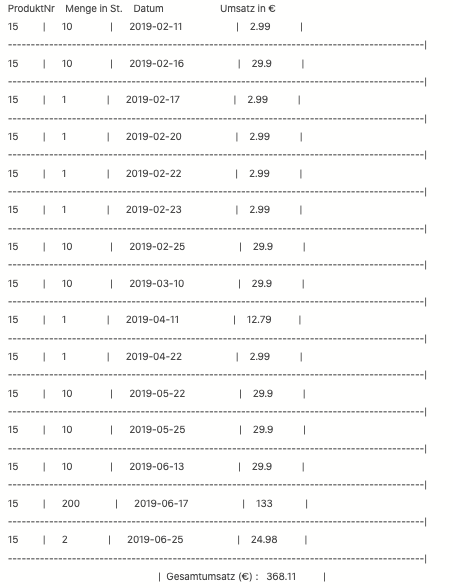
\includegraphics[width=1.1\linewidth]{pictures/report_sql.png}
  \caption{Reporting-Tabelle}
  \label{report_sql}
\end{figure}

Die Tabelle zeigt die Umsätze und die verkauften Mengen für die Produktnummer 15 in einem Zeitraum von 6 Monaten. Zunächst wird überprüft, ob die angegebenen Zeiten einen Zeitraum darstellen. Wenn die Differenz nicht negativ ist, beginnt der Insert der Daten aus der Kassenbon\_Faktentabelle in die Hilfstabelle. Der Cursor KB\_Cursor durchläuft jeden Tag mithilfe der Inkrementierung des Cursor-Status um 1. Wenn alle keine weiteren Verkäufe mehr für den Zeitraum und das Produkt gefunden werden, wird die Schleife beendet. Anschließend wird der Gesamtumsatz berechnet und der Cursor wird beendet.

\subsection{Reporting mit QlikSense}

Neben der Auswertung mit Prozeduren kann eine Datenauswertung mit der BI-Sofwtware QlikSense durchgeführt werden. Der Vorteil ist die bessere Visualisierung in anschaulichen Diagrammen.

\subsubsection{Produkte nach Umsätzen}

Im folgenden Kreisdiagramm wird dargestellt, welche Produkte insgesamt die umsatzstärksten sind. Es wurde nach der Dimension Produktbezeichnung und der Kennzahl sum(Umsatz) erstellt. Die Geschäftsführer können somit die Erkenntniss gewinnen, dass der Bacardi Carta Blanca z.B. länger im Sortiment behalten werden kann. Dagegen kann aus Abbildung \ref{produktearm} entnommen werden, welche Produkte z.B. aus dem Sortiment genommen, besser beworben oder besser platziert müssen.

\begin{figure}[H]
  \centering
  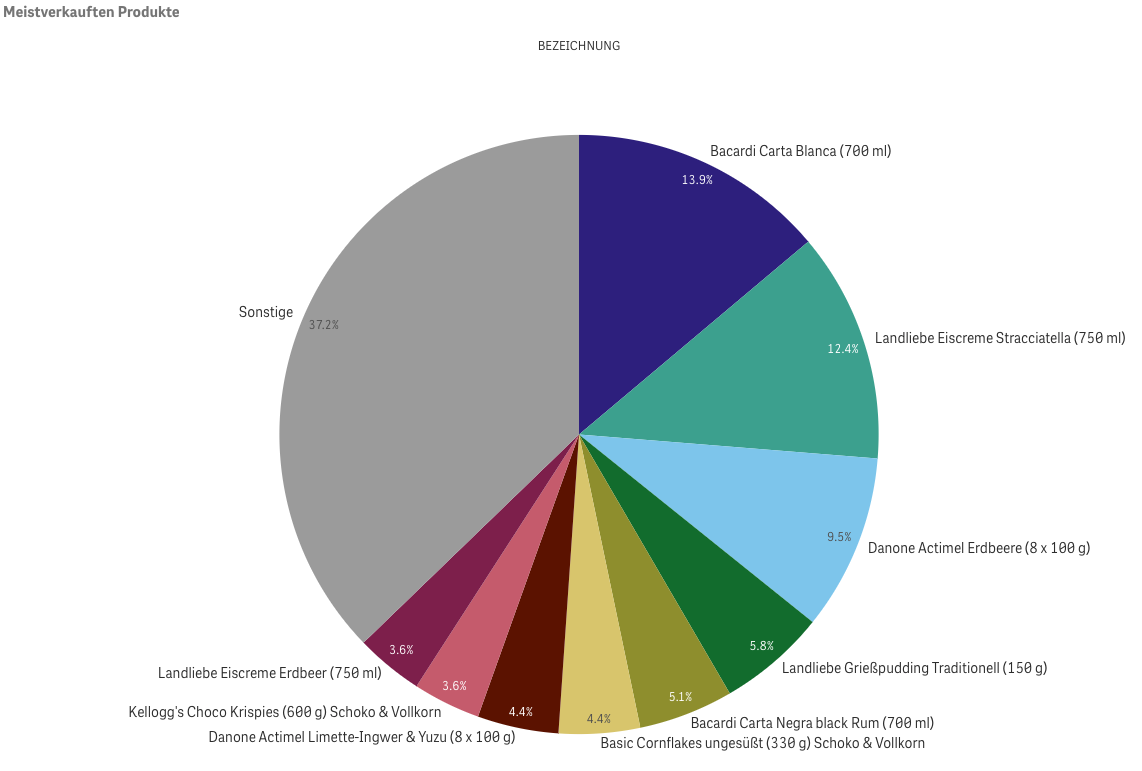
\includegraphics[width=1.2\linewidth]{pictures/meistverkauft_produkt.png}
  \caption{Umsatzstärksten Produkte}
  \label{produkte}
\end{figure}
\begin{figure}[H]
  \centering
  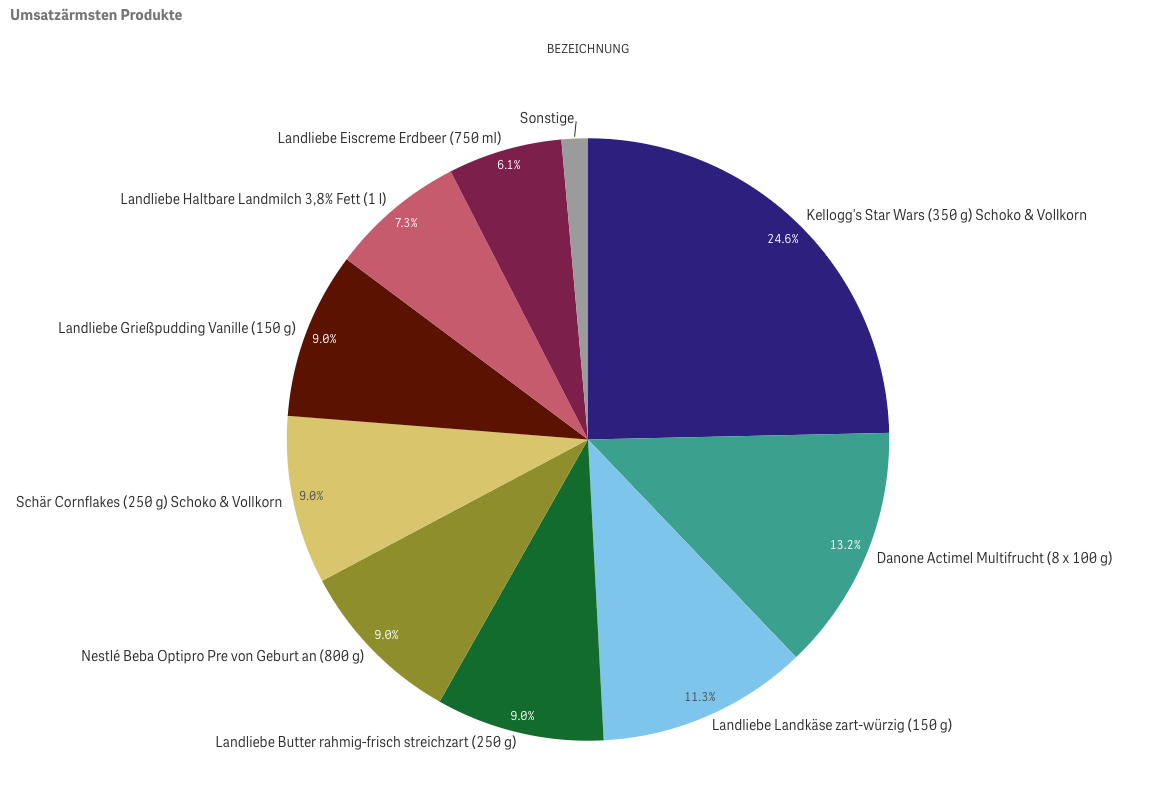
\includegraphics[width=1.2\linewidth]{pictures/umsatzarm.png}
  \caption{Umsatzärmsten Produkte}
  \label{produktearm}
\end{figure}
\subsubsection{Erfolgreichsten Handelsmarken}

Diese Analyse zeigt die größten Umsätze nach Handelsmarken. Wie aus der Produktanalyse ersichtlich ist, ist Bacardi eine sehr erfolgreiche Marke im Verkauf. Auch die Marken Danone und Landliebe haben großes Potenzial. Daraus kann geschlossen werden, dass die Kunden großes Interesse an den Produkten haben können, wenn z.B. bessere Werbe- oder Platzierungsmaßnahmen ergriffen werden, aber auch Produktvariationen erstellt werden.

\begin{figure}[H]
  \centering
  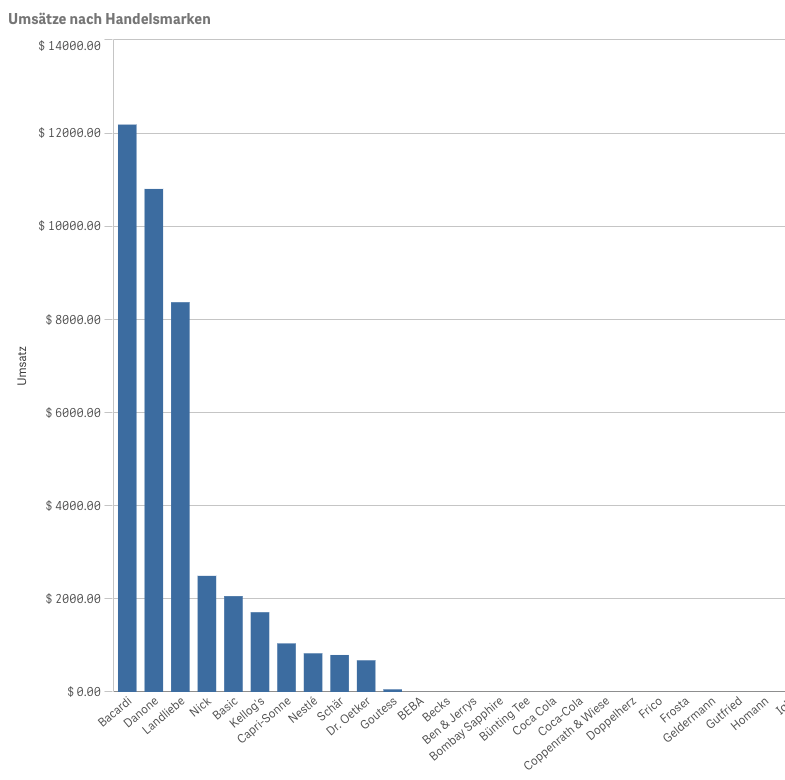
\includegraphics[width=1.1\linewidth]{pictures/ums_handelsmarke.png}
  \caption{Erfolgreichsten Handelsmarken}
  \label{kw}
\end{figure}

\subsubsection{Auswertung nach Kalenderwochen}

Dieses Diagramm berücksichtigt die Dimension Kalenderwoche nach den durschnittlich verkauften Mengen und entsprechenden Umsätzen. Daraus kann man entnehmen, dass die Kalenderwoche 7 die erfolgreichste war. Die Geschäftsführung könnte sich Gedanken darum machen, welche Ereignisse diesen Erfolg begründen könnten.

\begin{figure}[H]
  \centering
  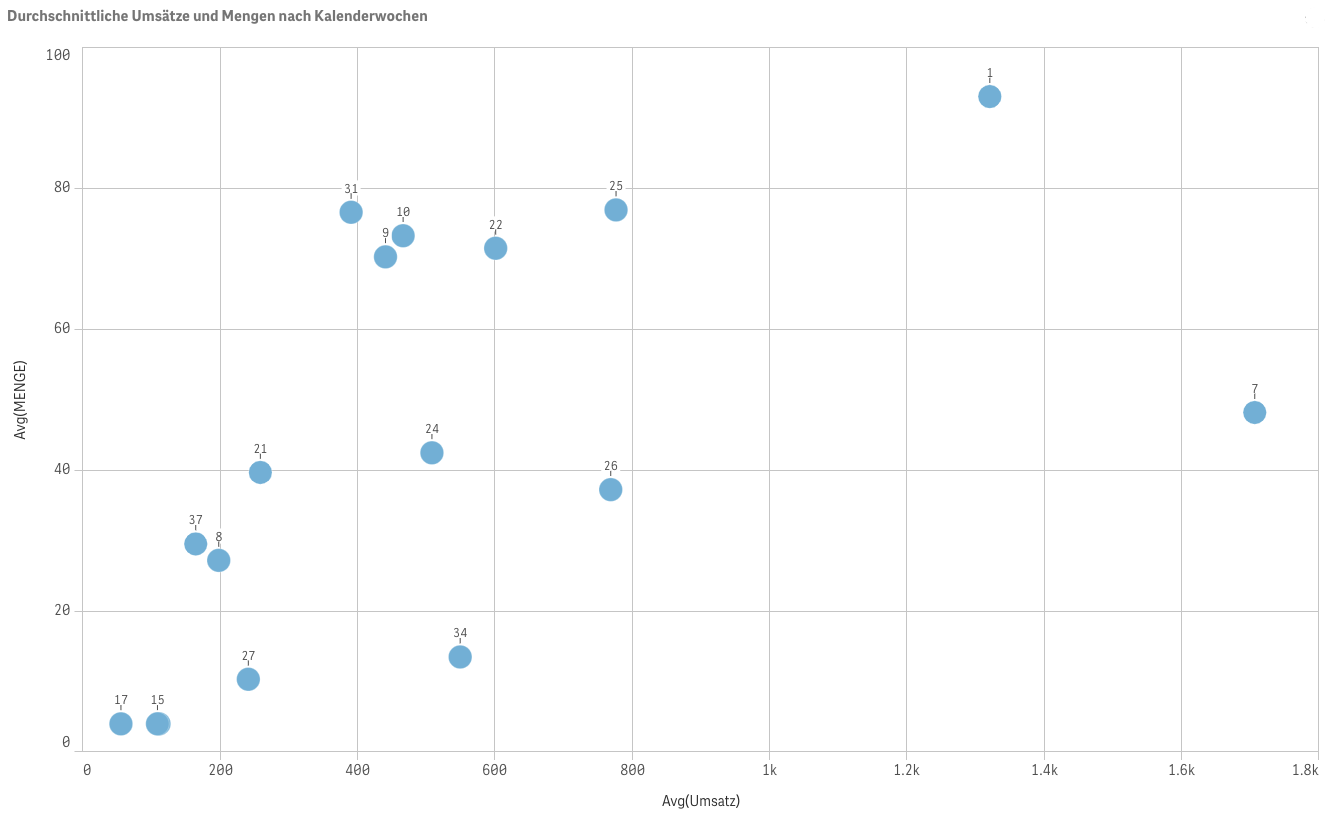
\includegraphics[width=1.2\linewidth]{pictures/kalenderwochen.png}
  \caption{Umsätze und Mengen nach Kalenderwochen}
  \label{kw}
\end{figure}

\newpage

